\documentclass[12pt,a4paper,conference]{IEEEtran}
\usepackage[utf8]{inputenc}
\usepackage[english]{babel}
\usepackage{amsmath}
\usepackage{amsfonts}
\usepackage{amssymb}
\usepackage{graphicx}

\usepackage{float}
\usepackage{fullpage}

\usepackage{hyperref}

\usepackage{tikz}

\usepackage{todonotes}
\usepackage{epstopdf}
\usepackage{graphicx}
\usepackage[T1]{fontenc}


\let\ig\includegraphics
\renewcommand{\includegraphics}[2][]{ \IfFileExists{#2}{ \ig[#1]{#2} }{ 
		\IfFileExists{#2.eps}{ \ig[#1]{#2} }{ 
		\IfFileExists{#2.png}{ \ig[#1]{#2} }{ 
		\IfFileExists{#2.jpg}{ \ig[#1]{#2} }{ 
		\IfFileExists{#2.jpeg}{ \ig[#1]{#2} }{ 
		\IfFileExists{#2.gif}{ \ig[#1]{#2} }{ 
		\IfFileExists{#2.ppm}{ \ig[#1]{#2} }{ 
		\missingfigure{  \protect\detokenize{#2} was not found.} 
}}}}}}}
}

\newcommand{\missingequation}[1]{\todo[inline, color = yellow]{Missing equation: #1}}


%%
%% End of file `mypackage.sty'.

\begin{document}
\raggedbottom

\title{Image Restoration\\ \large{ROVI - Miniproject}}
\author{Nicolaj Iversen and Lukas Schwartz}
\date{9$^{th}$ November 2015}

\maketitle

\section{Image Restoration}
This report sets to describe the how the four given images from the ROVI lecture are restored to better display the image content.
Each image is separately dealt with in each their section.

For simplicity, three areas/zones of the images are defined beforehand to display results and analyse sub-areas of the image.
These three parts are called uniform, complex and simple area.
Where complex is a cutout of the fingers of the robot, uniform is a blank surface for which the image should contain only one uniform color and simple is \textbf{WHAT?} .


\subsection{Pepper Noise}\label{image_1}
Pepper noise is when a set of pixels on an image are complete black, without the actual photographed scene has these elements.
To find the noise in an image, an uniform area is selected and analysed.
In figure \ref{fig:hist_pepper_im01} can it be seen that the image suffers from pepper noise.
It is assumed that the proportion of pepper in the uniform area is the same as over the whole of the image.

\begin{figure}[H]
\centering

\includegraphics[width = \histogramWidth]{graphics/hist1_uniform.png}
\caption{Histogram of the original ``Image1.png'' showing pepper noise in a uniform area.}
\label{fig:hist_pepper_im01}
\end{figure}

A median filter is good to combat salt and pepper noise as it takes the midpoint and thus avoids extreme values.
This assumes that the amount of salt or pepper is less than 20\% and the filter is large enough to get values which are neither entire salt or entire pepper.
To remove pepper noise from an image with mostly pepper noise, the amount of pepper damage needs to be found.
The image was detected to be 60\% pepper.
This means a median filter is not viable as the midpoint is likely to turn out as pepper.

Knowing this means that the midpoint must be shifted towards a lighter color.
This method is called alpha trimmed mean.
The new midpoint which can be calculated using equation \ref{eq:quantile} and was found to be 80\%. 

\begin{equation}
 q = (\text{pepper}-\text{salt}+1)/2 \label{eq:quantile}
\end{equation}

A 3x3 midpoint filter is applied to the image to remove the majority of the damage to the image.
Then a 7x7 alpha trimmed mean with a width of 3 is applied to further remove the pepper noise.
Running a median filter twice gives the effect of overestimating the damage of the pepper and thus results in a brighter image.

To see if the filters does damage to the original image an area with more complex features are shown.
In figure \ref{fig:complex1_after_alpha} can the area be seen after the alpha trimmed mean filter has been applied.
It can be seen that there is still noise present in the image.

\begin{figure}[H]
\centering
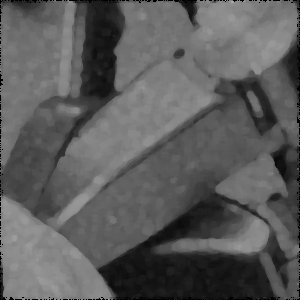
\includegraphics[width = \cutOutWidth]{graphics/complex1_step2}
\caption{Image in a complex area after alpha trimmed mean filter.}
\label{fig:complex1_after_alpha}
\end{figure}

To see the noise, another histogram of the uniform area is made.
In figure \ref{fig:hist_img1_after_alpha} can the histogram of the uniformed area after the applying two filters be seen.
The histogram suggest that there is still Gaussian noise in the image.
Gaussian noise can be removed by applying an arithmetic mean filter.

\begin{figure}[H]
\centering
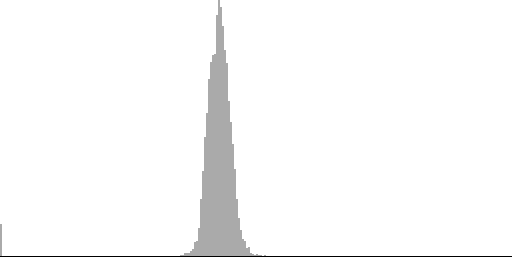
\includegraphics[width = \histogramWidth]{graphics/hist1_uniform2.png}
\caption{Histogram of the filtered uniform area after alpha trimmed mean filter.}
\label{fig:hist_img1_after_alpha}
\end{figure}

In figure \ref{fig:complex1_after_blur} can the effect of applying arithmetic mean to the image be seen.
By taking the image into logarithmic space, the noise becomes additive and thus can be separated with a arithmetic mean filter.
In figure \ref{fig:complex1_after_harmonic} can the effect of using a harmonic mean arithmetic mean filter be seen.
Both filters have the size of 5x5. The Difference is not that obvious from visual inspection so the difference is calculated using equation \ref{eq:img_diff_harVSgeo}.

\begin{equation}
I_{diff} = \left( I_{har} - I_{geo} \right) * A + 127
\label{eq:img_diff_harVSgeo}
\end{equation}

The difference is shown in figure \ref{fig:complex1_blur_difference}.
The difference is amplified 50 times in order to get a clear contrast between the two.
Darker areas means regular blurring contains higher values.
The most distinct difference between the images is the edges. 
The edges are brighter after the regular filter. 
The most visible edges on the difference image occurs where the image goes from a large area of light to a small area of dark.
Thus the edges are better preserved on the harmonic mean filter.
In the lower right corner, the underside of the gripper is supposed to be dark.
Therefore having higher values with the regular filter gives unwanted bright spots which the harmonic mean filter removes.
It is therefore concluded that the harmonic mean filter is the best for this task.



\begin{figure}[H]
\centering
  \begin{subfigure}{\linewidth}
  \centering
    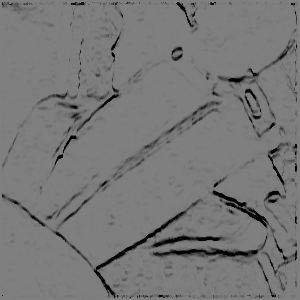
\includegraphics[width = \cutOutWidth]{graphics/complex1_blurr_difference_50.png}
    \caption{Difference.}
    \label{fig:complex1_blur_difference}
  \end{subfigure}
  
  \begin{subfigure}{\cutOutWidth}
    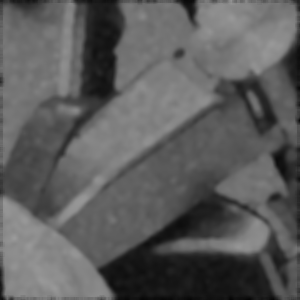
\includegraphics[width = \textwidth]{graphics/complex1_blurred.png}
    \caption{Geometric Mean.}
    \label{fig:complex1_after_blur}
  \end{subfigure}
%
  \begin{subfigure}{\cutOutWidth}
    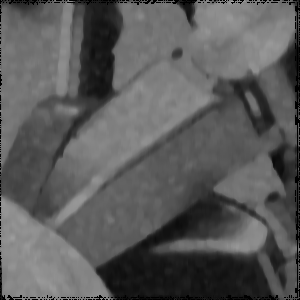
\includegraphics[width = \textwidth]{graphics/complex1_harmonic_blurred.png}
    \caption{Harmonic mean.}
    \label{fig:complex1_after_harmonic}
  \end{subfigure}
\caption{Image in a complex area after applying different mean filters.}
\end{figure}

The resulting sequence is thus:
\begin{itemize}
 \item Shifted midpoint filter, kernel size 3x3, quantile of 80\%.
 \item Alpha mean filter, kernel size 7x7, quantile of 80\%, mean width of 3.
 \item Harmonic mean filter, kernel size 5x5.
\end{itemize}

The final image of image 1 can be seen in figure \ref{fig:final_image1}.

\begin{figure}[H]
\centering
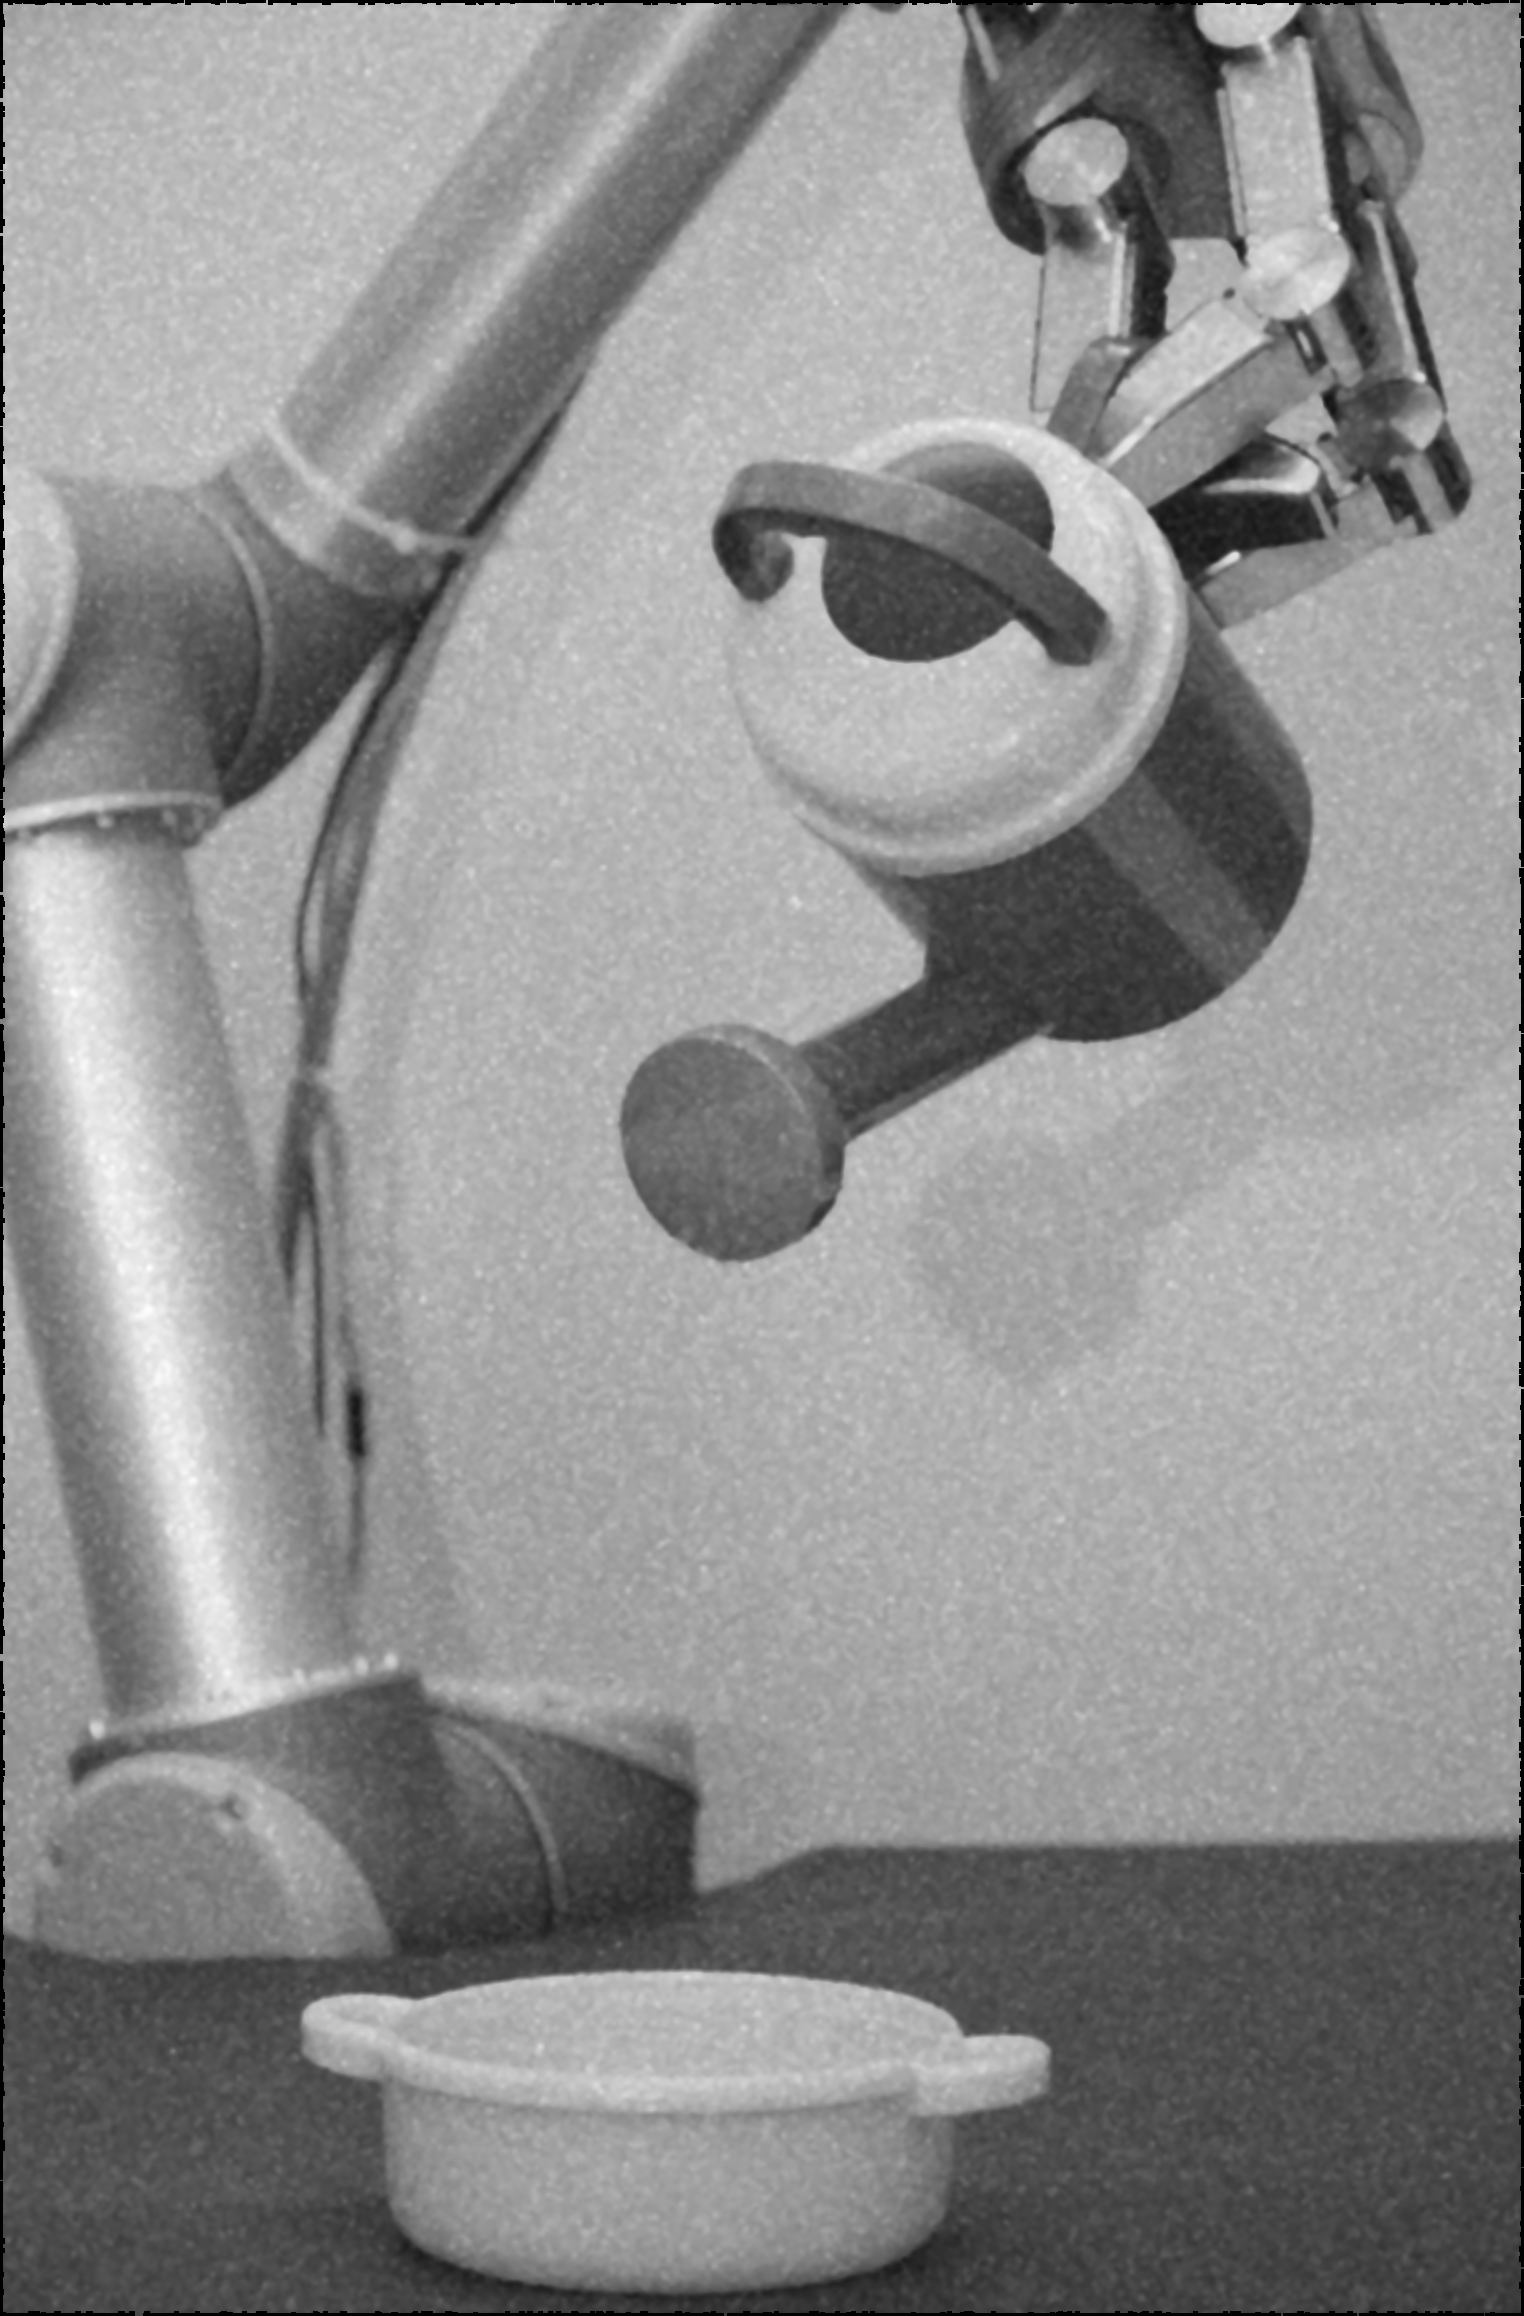
\includegraphics[width = \fullImageWidth]{../code/images/image_result_1.png}
\caption{Image 1 restored.}
\label{fig:final_image1}
\end{figure}


\subsection{Gaussian Noise with Salt and Pepper}

By analyzing image 2 in an uniform area it can be seen that the image has both salt and pepper noise, illustrated in figure \ref{fig:hist2_uniform}.
As in section \ref{image_1} this is removed with a shifted median filter. 
It was found that a 5x5 filter removed the extreme values but was not efficient at removing the rest of the noise.

\begin{figure}[H]
\centering
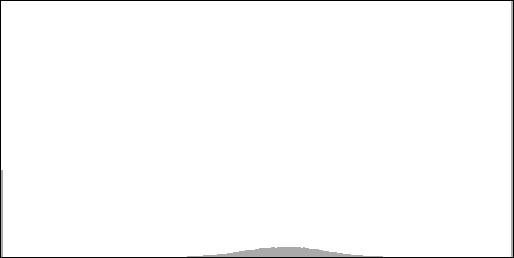
\includegraphics[width = \histogramWidth]{graphics/hist2_uniform.png}
\caption{Histogram of the original ``Image2.png'' showing salt and pepper noise in a uniform area.}
\label{fig:hist2_uniform}
\end{figure}

Thus a harmonic mean filter is used to remove the remaining salt noise.
In figure \ref{fig:hist2_median} can it be seen that the removal of salt and pepper noise was successful.

\begin{figure}[H]
\centering
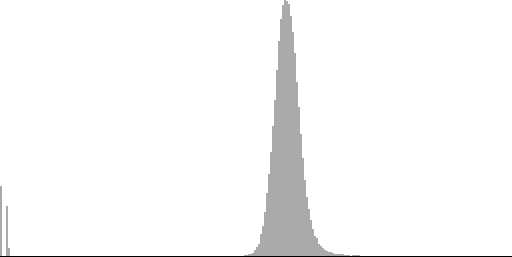
\includegraphics[width = \histogramWidth]{graphics/hist2_after_median.png}
\caption{Histogram of the uniform area after median filter.}
\label{fig:hist2_median}
\end{figure}

Gaussian noise remains and this was removed with a homomorphic bilateral filter.
In figure \ref{fig:hist2_bilateral} can it be seen that the variance has decreased.

\begin{figure}[H]
\centering
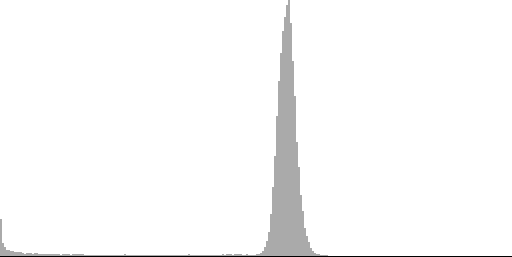
\includegraphics[width = \histogramWidth]{graphics/hist2_after_bilatteral.png}
\caption{Histogram of the uniform area after bilateral filter.}
\label{fig:hist2_bilateral}
\end{figure}

By analyzing a complex region, it can be seen that the image lacks contrast.
In figure \ref{fig:complex2_bilatteral} can the image be seen after a median filter and the homomorphic bilatteral filter.

\begin{figure}[H]
\centering
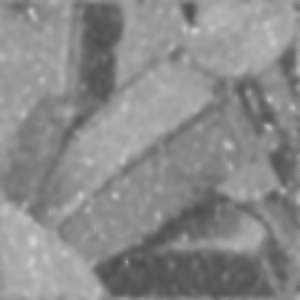
\includegraphics[width = \cutOutWidth]{graphics/complex2_bilatteral.png}
\caption{The complex area after bilatteral filter.}
\label{fig:complex2_bilatteral}
\end{figure}

The lack of contrast can be added with a histogram equalization scheme.
In figure \ref{fig:complex2_histeq} can the image be seen after histogram equalization.

\begin{figure}[H]
\centering
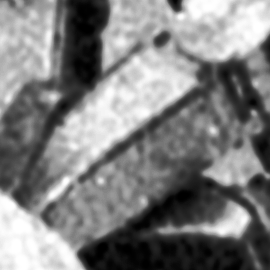
\includegraphics[width = \cutOutWidth]{graphics/complex2_histeq.png}
\caption{Histogram equalization of the complex area.}
\label{fig:complex2_histeq}
\end{figure}


The histogram equalization stretches the color values to the extremes and thus the image quality does not improve.
So before the histogram equalization, a alpha trimmed mean with the kernel size of 7x7 and mean width of 3 is applied to remove further extreme values.
In figure \ref{fig:complex2_histeq_smoothed} can the image be seen after alpha trimmed smoothed and then histogram equalization.

\begin{figure}[H]
\centering
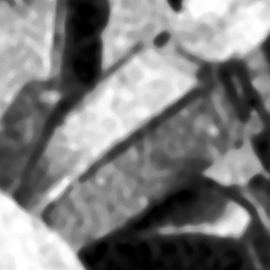
\includegraphics[width = \cutOutWidth]{graphics/complex2_histeq_smoothed.png}
\caption{Histogram equalization of the smoothed compex area.}
\label{fig:complex2_histeq_smoothed}
\end{figure}

The resulting image restoration of image 2 can be seen in figure \ref{fig:image_2_restored}.

\begin{figure}[H]
\centering
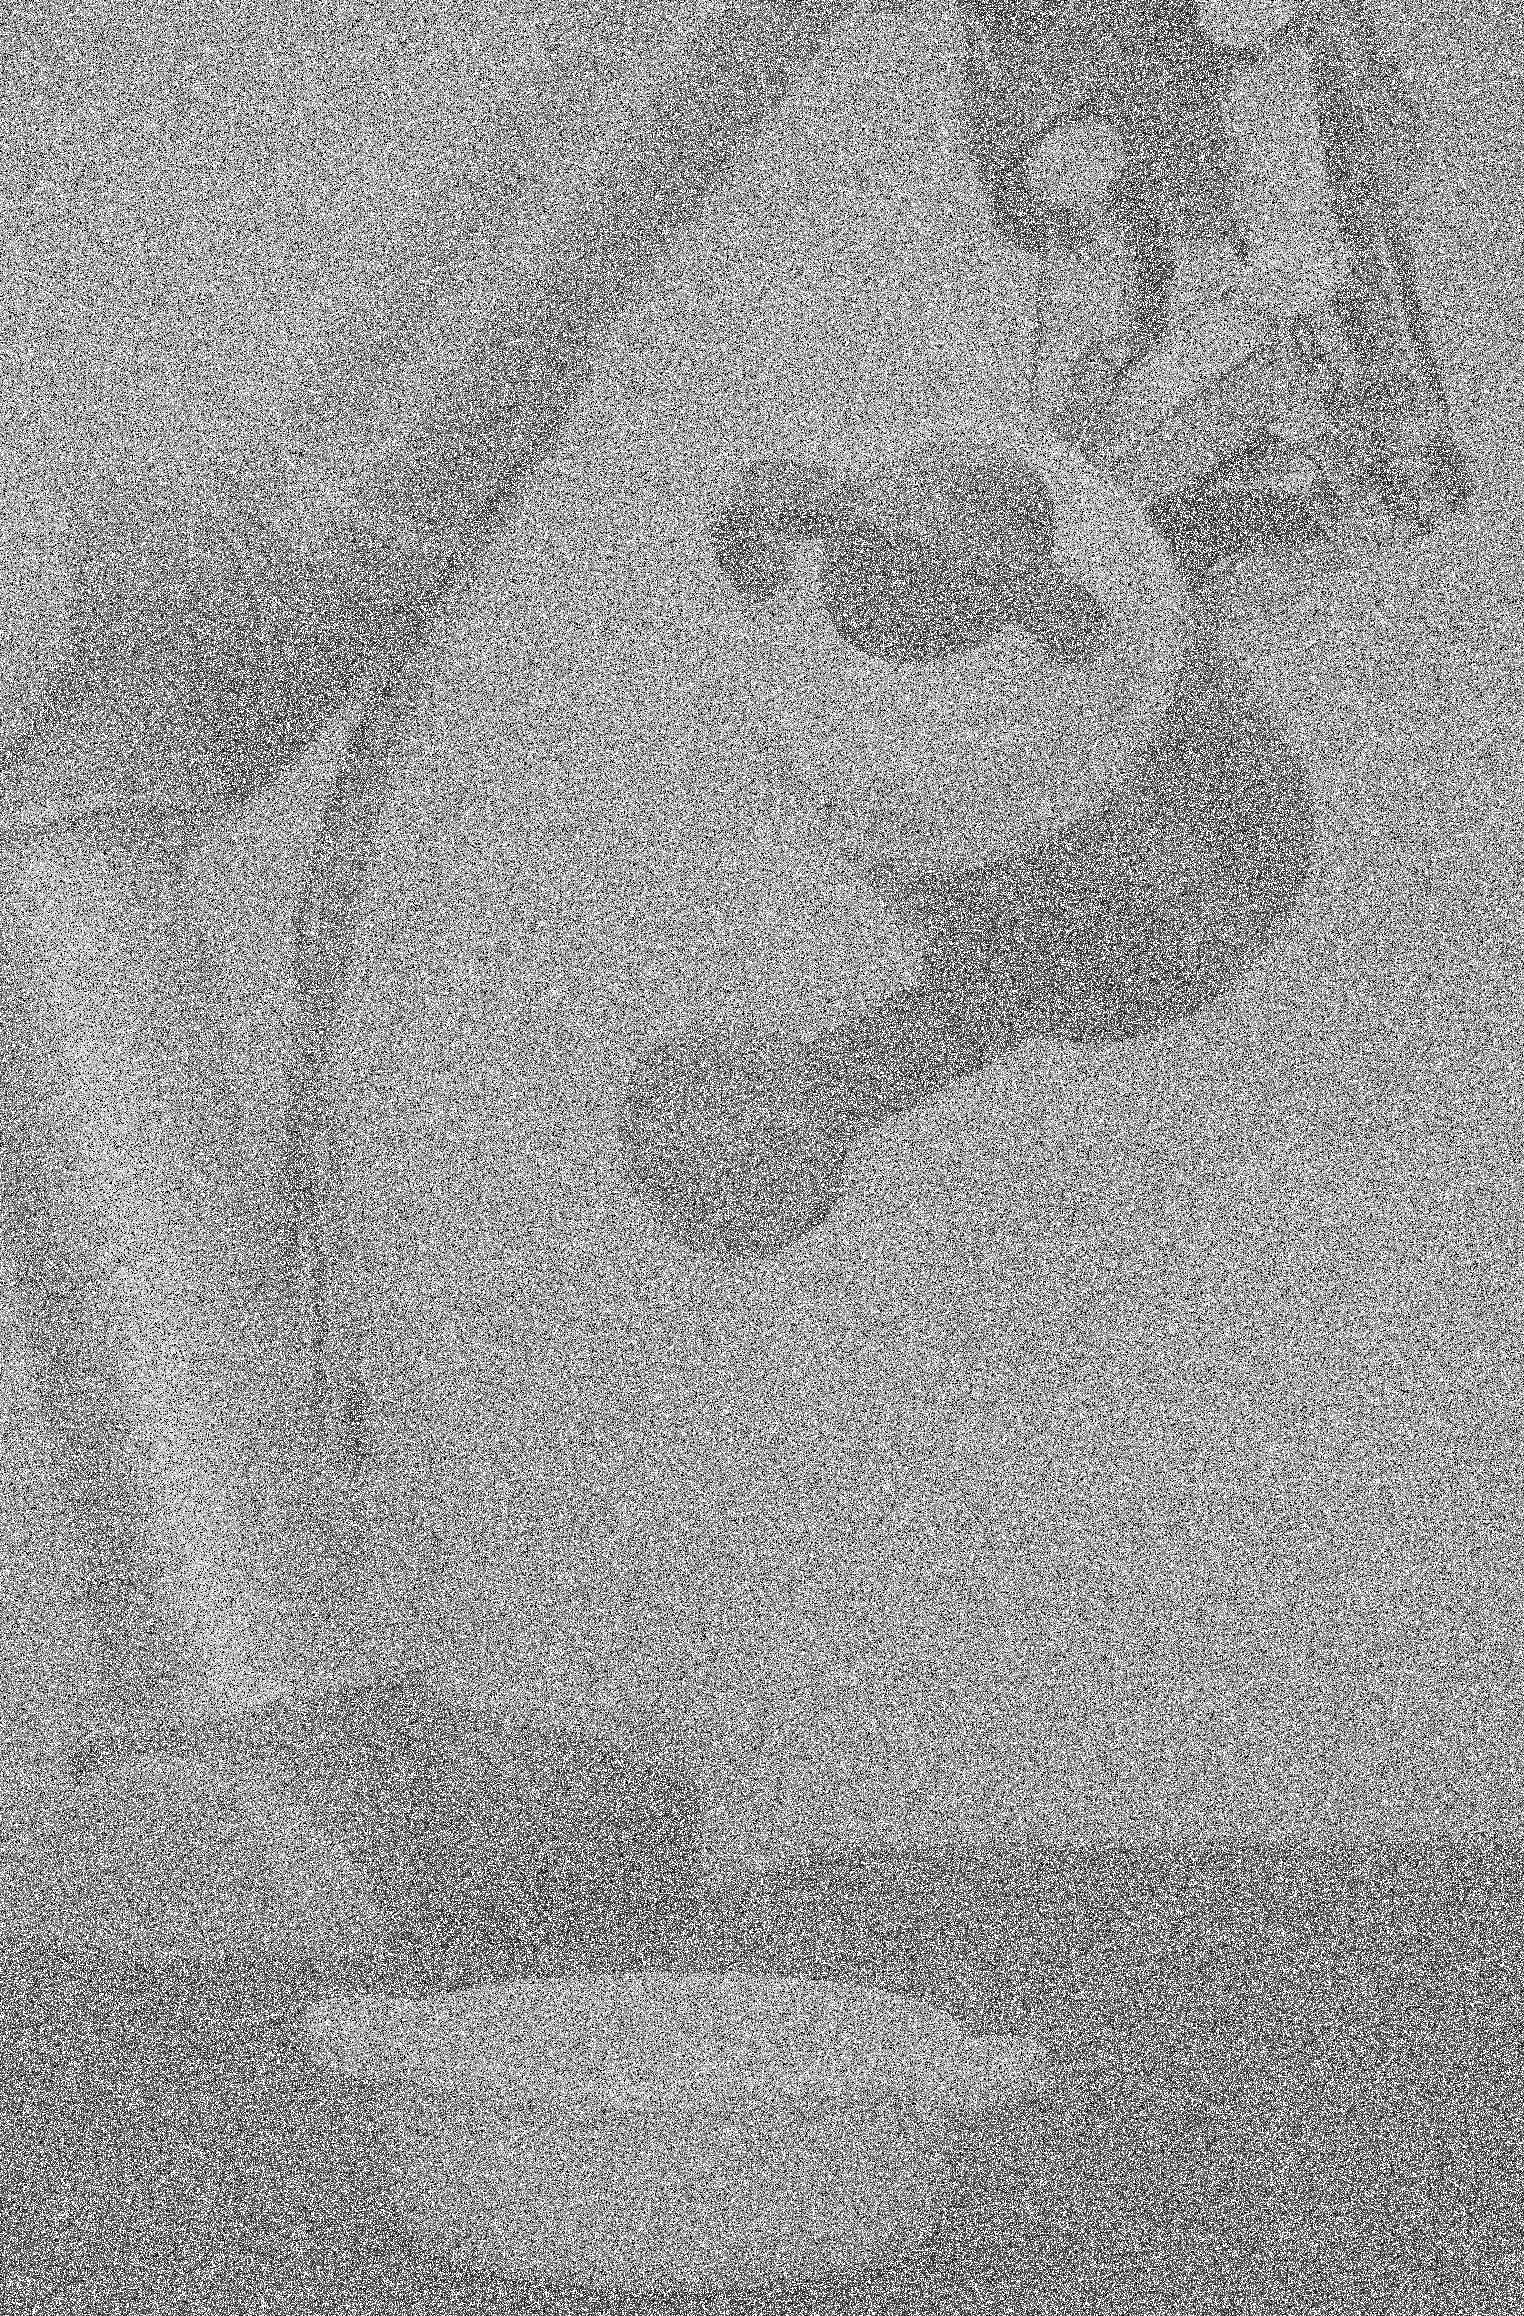
\includegraphics[width = \fullImageWidth]{../code/images/image_result_2.png}
\caption{The restored image 2.}
\label{fig:image_2_restored}
\end{figure}




\subsection{Gaussian/Uniform Noise}
To analyse the third image provided, a histogram of both the whole image and the uniform coloured area was computed.
This is seen in figure \ref{fig:hist_pre_im03} and \ref{fig:hist_uni_im03}.


\begin{figure}[H]
\centering
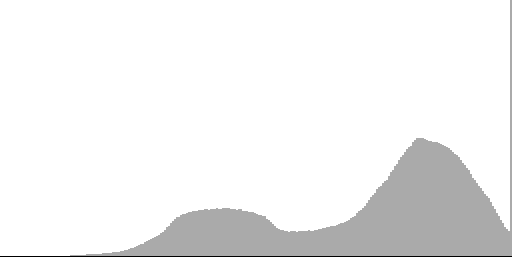
\includegraphics[width= 0.9 \linewidth]{../code/images/histogram_full_pre_03}
\caption{Histogram of the uniform area of image 3.}
\label{fig:hist_pre_im03}
\end{figure}

The histogram in figure \ref{fig:hist_pre_im03} shows that the image contains a large amount of light colors.
This should be corrected for to improve the visual appearance of the image.
Furthermore, when considering figure \ref{fig:hist_uni_im03}, then the image also contains a mix of Gaussian and uniform noise.
Uniform because of the flat top of the noise distribution in figure \ref{fig:hist_uni_im03} and Gaussian since the bell-shape-like curves on the two sides.


\begin{figure}[H]
\centering
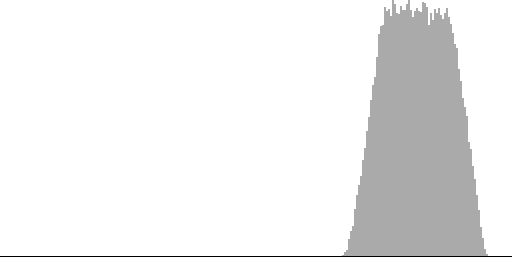
\includegraphics[width= 0.9 \linewidth]{../code/images/histogram_uniform_03}
\caption{Histogram of the full image 3.}
\label{fig:hist_uni_im03}
\end{figure}


In order to fix both problems in the image, a set of different approaches can be taken.
The intensity of the image can be improved by either using a histogram-equalization or an intensity correction.
The advantage of the former is that this would also improve the contrast of the image whereas the latter only adjusts the brightness.

When a visual inspection of the two approaches is made, it is clear that the image improves the most with the intensity correction.
This is because the histogram-equalization also affects the noise present in the image and spreads it out in a broader color range, making the damage look considerably more sever.
This is also the case when applying the histogram-equalization to the image after reducing the noise, with the method proposed for noise reduction below.
The magnitude of intensity correction was found by visual inspection to be -30 when the image has a depth of eight bits.


In order to reduce the Gaussian/uniform noise present in the image a mean filter is considered.
This is because it is additive noise and mean filters work well on those.

For this image the three mean filters arithmetic-, geometric- and harmonic mean filters were considered.
With visual inspection it is clear that the arithmetic filter performs considerably worse than the two other filters, geometric and harmonic.
When it comes to telling if the geometric or harmonic filters apart, it is not directly visible to the human eye which of the two resulting images are the best.
It was however found that a filter size of five gives a descend noise reduction, without blurring the information too much.

In order to compare the results from the geometric and harmonic images, the difference between the two in the complex area of the image is shown in figure \ref{fig:diff_harVSgeo_im03}.



\begin{figure}[H]
\centering
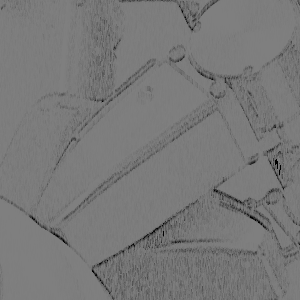
\includegraphics[width= 0.9 \linewidth]{../code/images/image_harVSgeo_complex_03}
\caption{Image difference between harmonic and geometric mean filtering in the complex area of image 3.}
\label{fig:diff_harVSgeo_im03}
\end{figure}


In figure \ref{fig:diff_harVSgeo_im03}, the amplified difference between the two images is plotted.
This was accomplished using equation \ref{eq:img_diff_harVSgeo}, where $I_{diff}$, $I_{har}$ and $I_{geo}$ is the intensity of the difference image, harmonic mean filtered and geometric mean filtered image respectively and $A$ is the scalar the difference is amplified with.

\begin{equation}
I_{diff} = \left( I_{har} - I_{geo} \right) * A + 127
\label{eq:img_diff_harVSgeo}
\end{equation}

For this image a $A$ of five was used.
Figure \ref{fig:diff_harVSgeo_im03} displays in dark/black the pixels of which the geometric mean filter gave the highest return, white for which it was the harmonic and grey for the values which are approximately equal.

It can from this be concluded that the geometric filter preserves the edges, as expected, more than the harmonic mean filter.
Therefore it was decided to use the geometric mean filter to restore the image.


\begin{figure}[H]
\centering
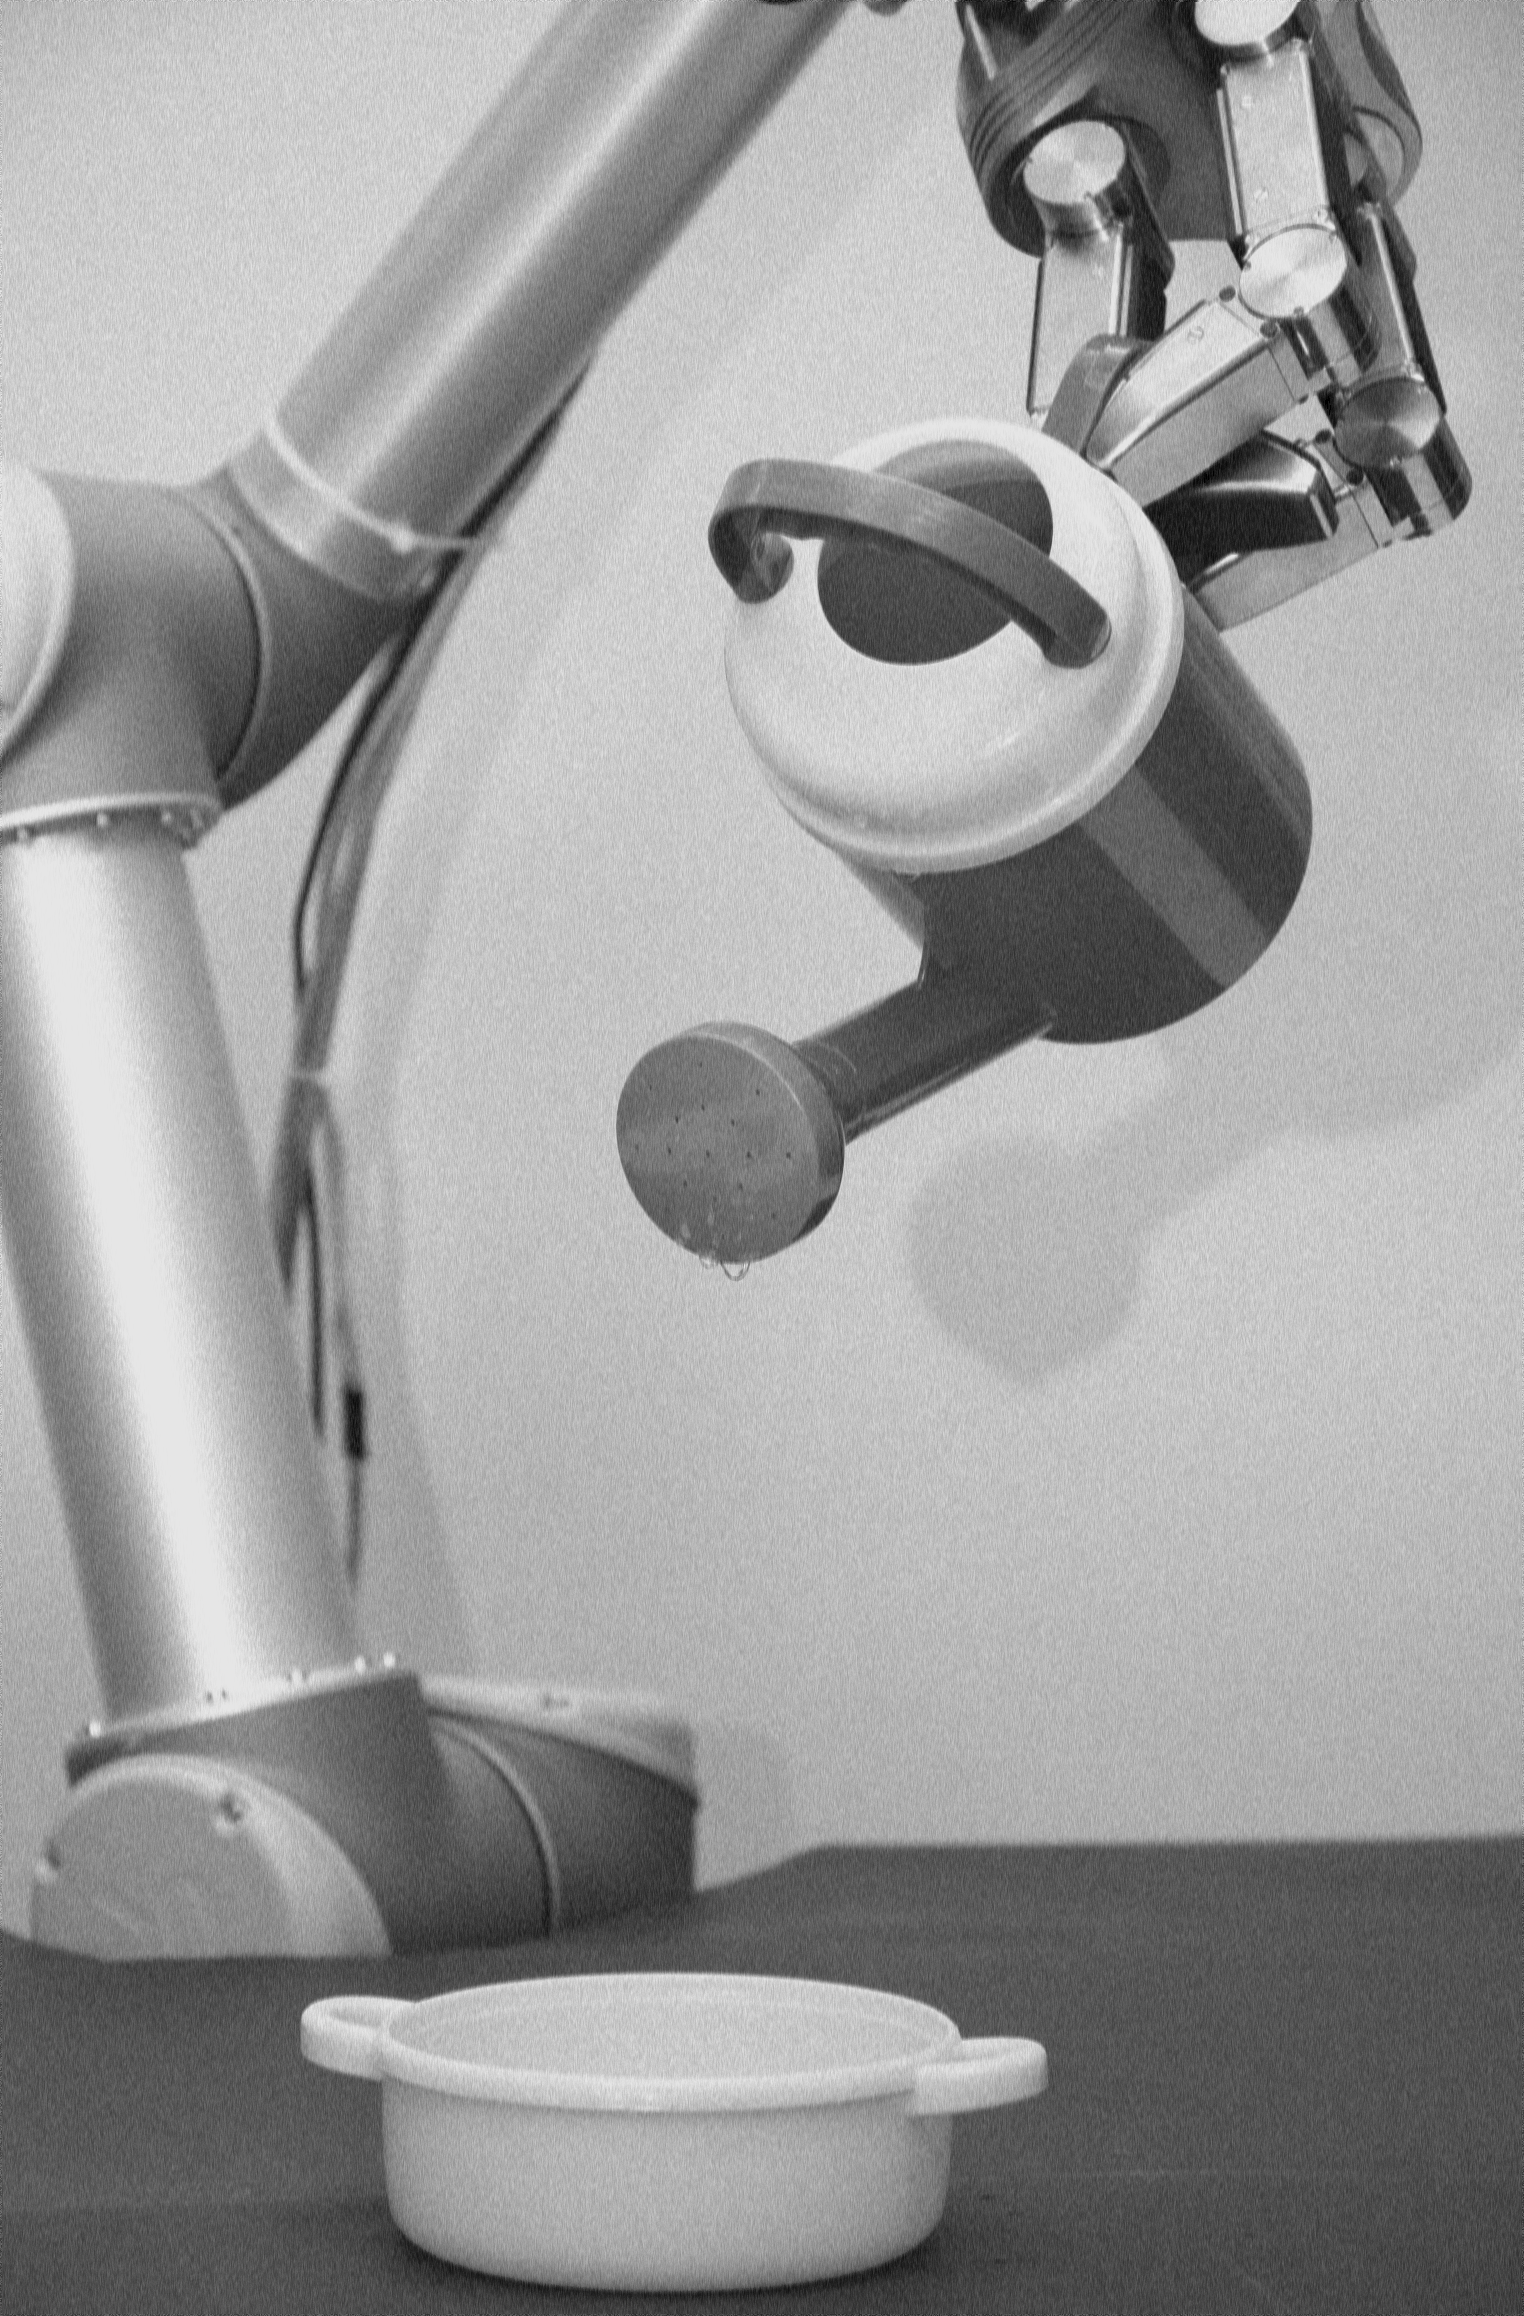
\includegraphics[width= 0.9 \linewidth]{../code/images/image_geometrical_03}
\caption{Resulting image after filtering using the geometric mean and kernel size of five on image 3 with intensity correction.}
\label{fig:img_result_im03}
\end{figure}


The resulting picture using both the intensity adjustment and geometric filter is seen in figure \ref{fig:img_result_im03}.
%From here both the histogram of the full image and the uniform area of the image is plotted resulting in figure \ref{fig:hist_post_im03} and \ref{fig:hist_uni_geo_im03} respectively.
The histogram of the uniform area of the resulting image is plotted in figure  \ref{fig:hist_uni_geo_im03}.


\begin{figure}[H]
\centering
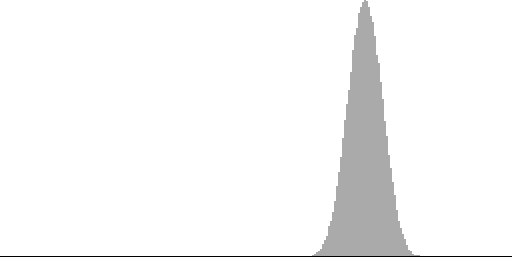
\includegraphics[width= 0.9 \linewidth]{../code/images/histogram_uniform_geometrical_03}
\caption{Histogram of the uniform area of image 3 after applying geometric mean filter with kernel size of five.}
\label{fig:hist_uni_geo_im03}
\end{figure}


It can from figure \ref{fig:hist_uni_geo_im03} be seen that the process correctly shifts the mean to the left, by the amount chosen for the intensity correction, and then filters the image into a narrower normal distribution than that seen in figure \ref{fig:hist_uni_im03}, yielding a visually better image than initially.





%\begin{figure}[H]
%\centering
%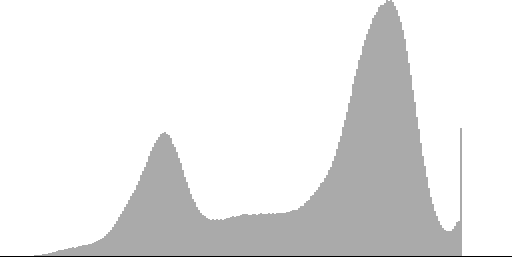
\includegraphics[width= 0.9 \linewidth]{../code/images/histogram_full_post_03}
%\caption{Histogram of the full resulting image 3.}
%\label{fig:hist_post_im03}
%\end{figure}


\subsection{Frequency Noise}
In this section image 4.1 is considered.
As the image contains a lot of disturbance in form of lines, a frequency analysis of the image was made.
The magnitude plot of a cutout of the uniform area of image 4.1 is seen in figure \ref{fig:freq_analysis_uni_p4} and the magnitude plot for the whole image in \ref{fig:freq_analysis_p4}.



\begin{figure}[H]
\centering
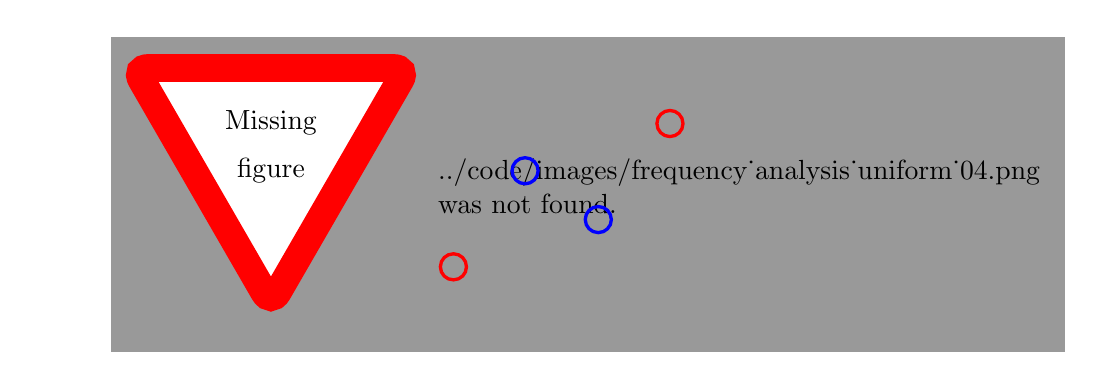
\begin{tikzpicture}
\node {\includegraphics[width = \fullImageWidth]{../code/images/frequency_analysis_uniform_04.png}};

\node[circle, draw, minimum width = 0.3cm,red,very thick] at (1.45, 0.9) {};

\node[circle, draw, minimum width = 0.3cm,red,very thick] at (-1.30, -0.92) {};

\node[circle, draw, minimum width = 0.3cm,blue,very thick] at (-0.39, 0.3) {};

\node[circle, draw, minimum width = 0.3cm,blue,very thick] at (0.54, -0.32) {};
\end{tikzpicture}
\caption{Magnitude plot of the uniform area of image 4.1 in the frequency domain.}
\label{fig:freq_analysis_uni_p4}
\end{figure}


\begin{figure}[H]
\centering
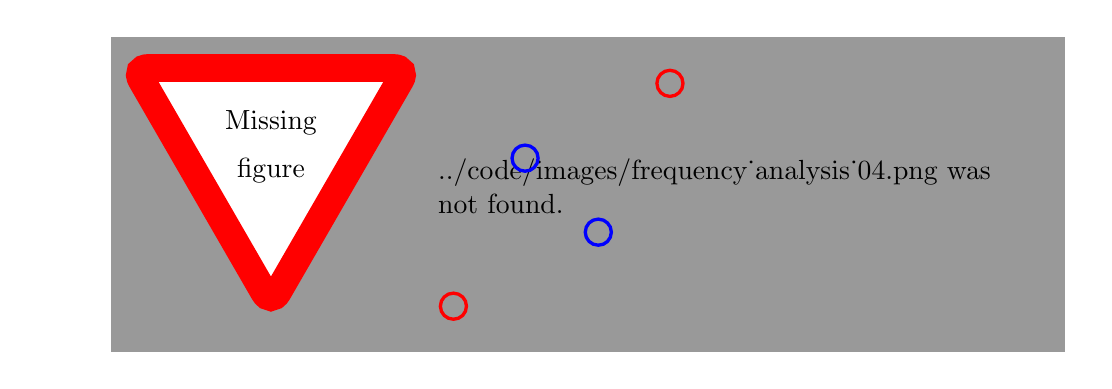
\begin{tikzpicture}

\node {\includegraphics[width = \fullImageWidth]{../code/images/frequency_analysis_04.png}};

\node[circle, draw, minimum width = 0.3cm,red,very thick] at (1.45, 1.41) {};

\node[circle, draw, minimum width = 0.3cm,red,very thick] at (-1.30, -1.42) {};

\node[circle, draw, minimum width = 0.3cm,blue,very thick] at (-0.39, 0.46) {};

\node[circle, draw, minimum width = 0.3cm,blue,very thick] at (0.54, -0.48) {};
\end{tikzpicture}

\caption{Magnitude plot of image 4.1 in the frequency domain.}
\label{fig:freq_analysis_p4}
\end{figure}


Figure \ref{fig:freq_analysis_uni_p4} is the frequency analysis of the uniform area of image 4.1.
This should ideally only contain the DC component when no noise is present.
It can therefore be concluded the the bright spots present on figure \ref{fig:freq_analysis_uni_p4}, apart from the DC component, must be caused by the disturbance.
These point pairs are circled on figure \ref{fig:freq_analysis_uni_p4} with each pair their own color.
The two disturbances originate from the lines at an approximate $\pm 45$ degrees angle from the horizon.

These points of disturbance can then be mapped directly onto the magnitude plot of the whole image.
In figure \ref{fig:freq_analysis_p4} the disturbance pairs are marked in the same color as on figure  \ref{fig:freq_analysis_uni_p4}.


In order to remove the disturbances, it was chosen to use a Butterworth filter located at the origin of the disturbances.
The cut-off frequency was chosen by testing a range of values and the best then chosen.

When the filters are applied to the image and the images is turned back into the spacial domain, figure \ref{fig:result_04} is gained.


\begin{figure}[H]
\centering
\includegraphics[width = \fullImageWidth]{../code/images/image_result_freq_04.png}
\caption{Resulting image after filtering the disturbance from image 4.1 in the frequency domain.}
\label{fig:result_04}
\end{figure}

Furthermore a new magnitude plot can be made, this is shown in figure \ref{fig:result_freq_04}.
It can here be seen that the points were not completely removed by the filter.
This is also visible on the resulting image, figure \ref{fig:result_04}, where the lines are still slightly visible in the borders of the image.
It can also be seen on figure \ref{fig:result_04} that the filtering introduced slight ringing effects around the bottom and outlet of the watering can.


\begin{figure}[H]
\centering
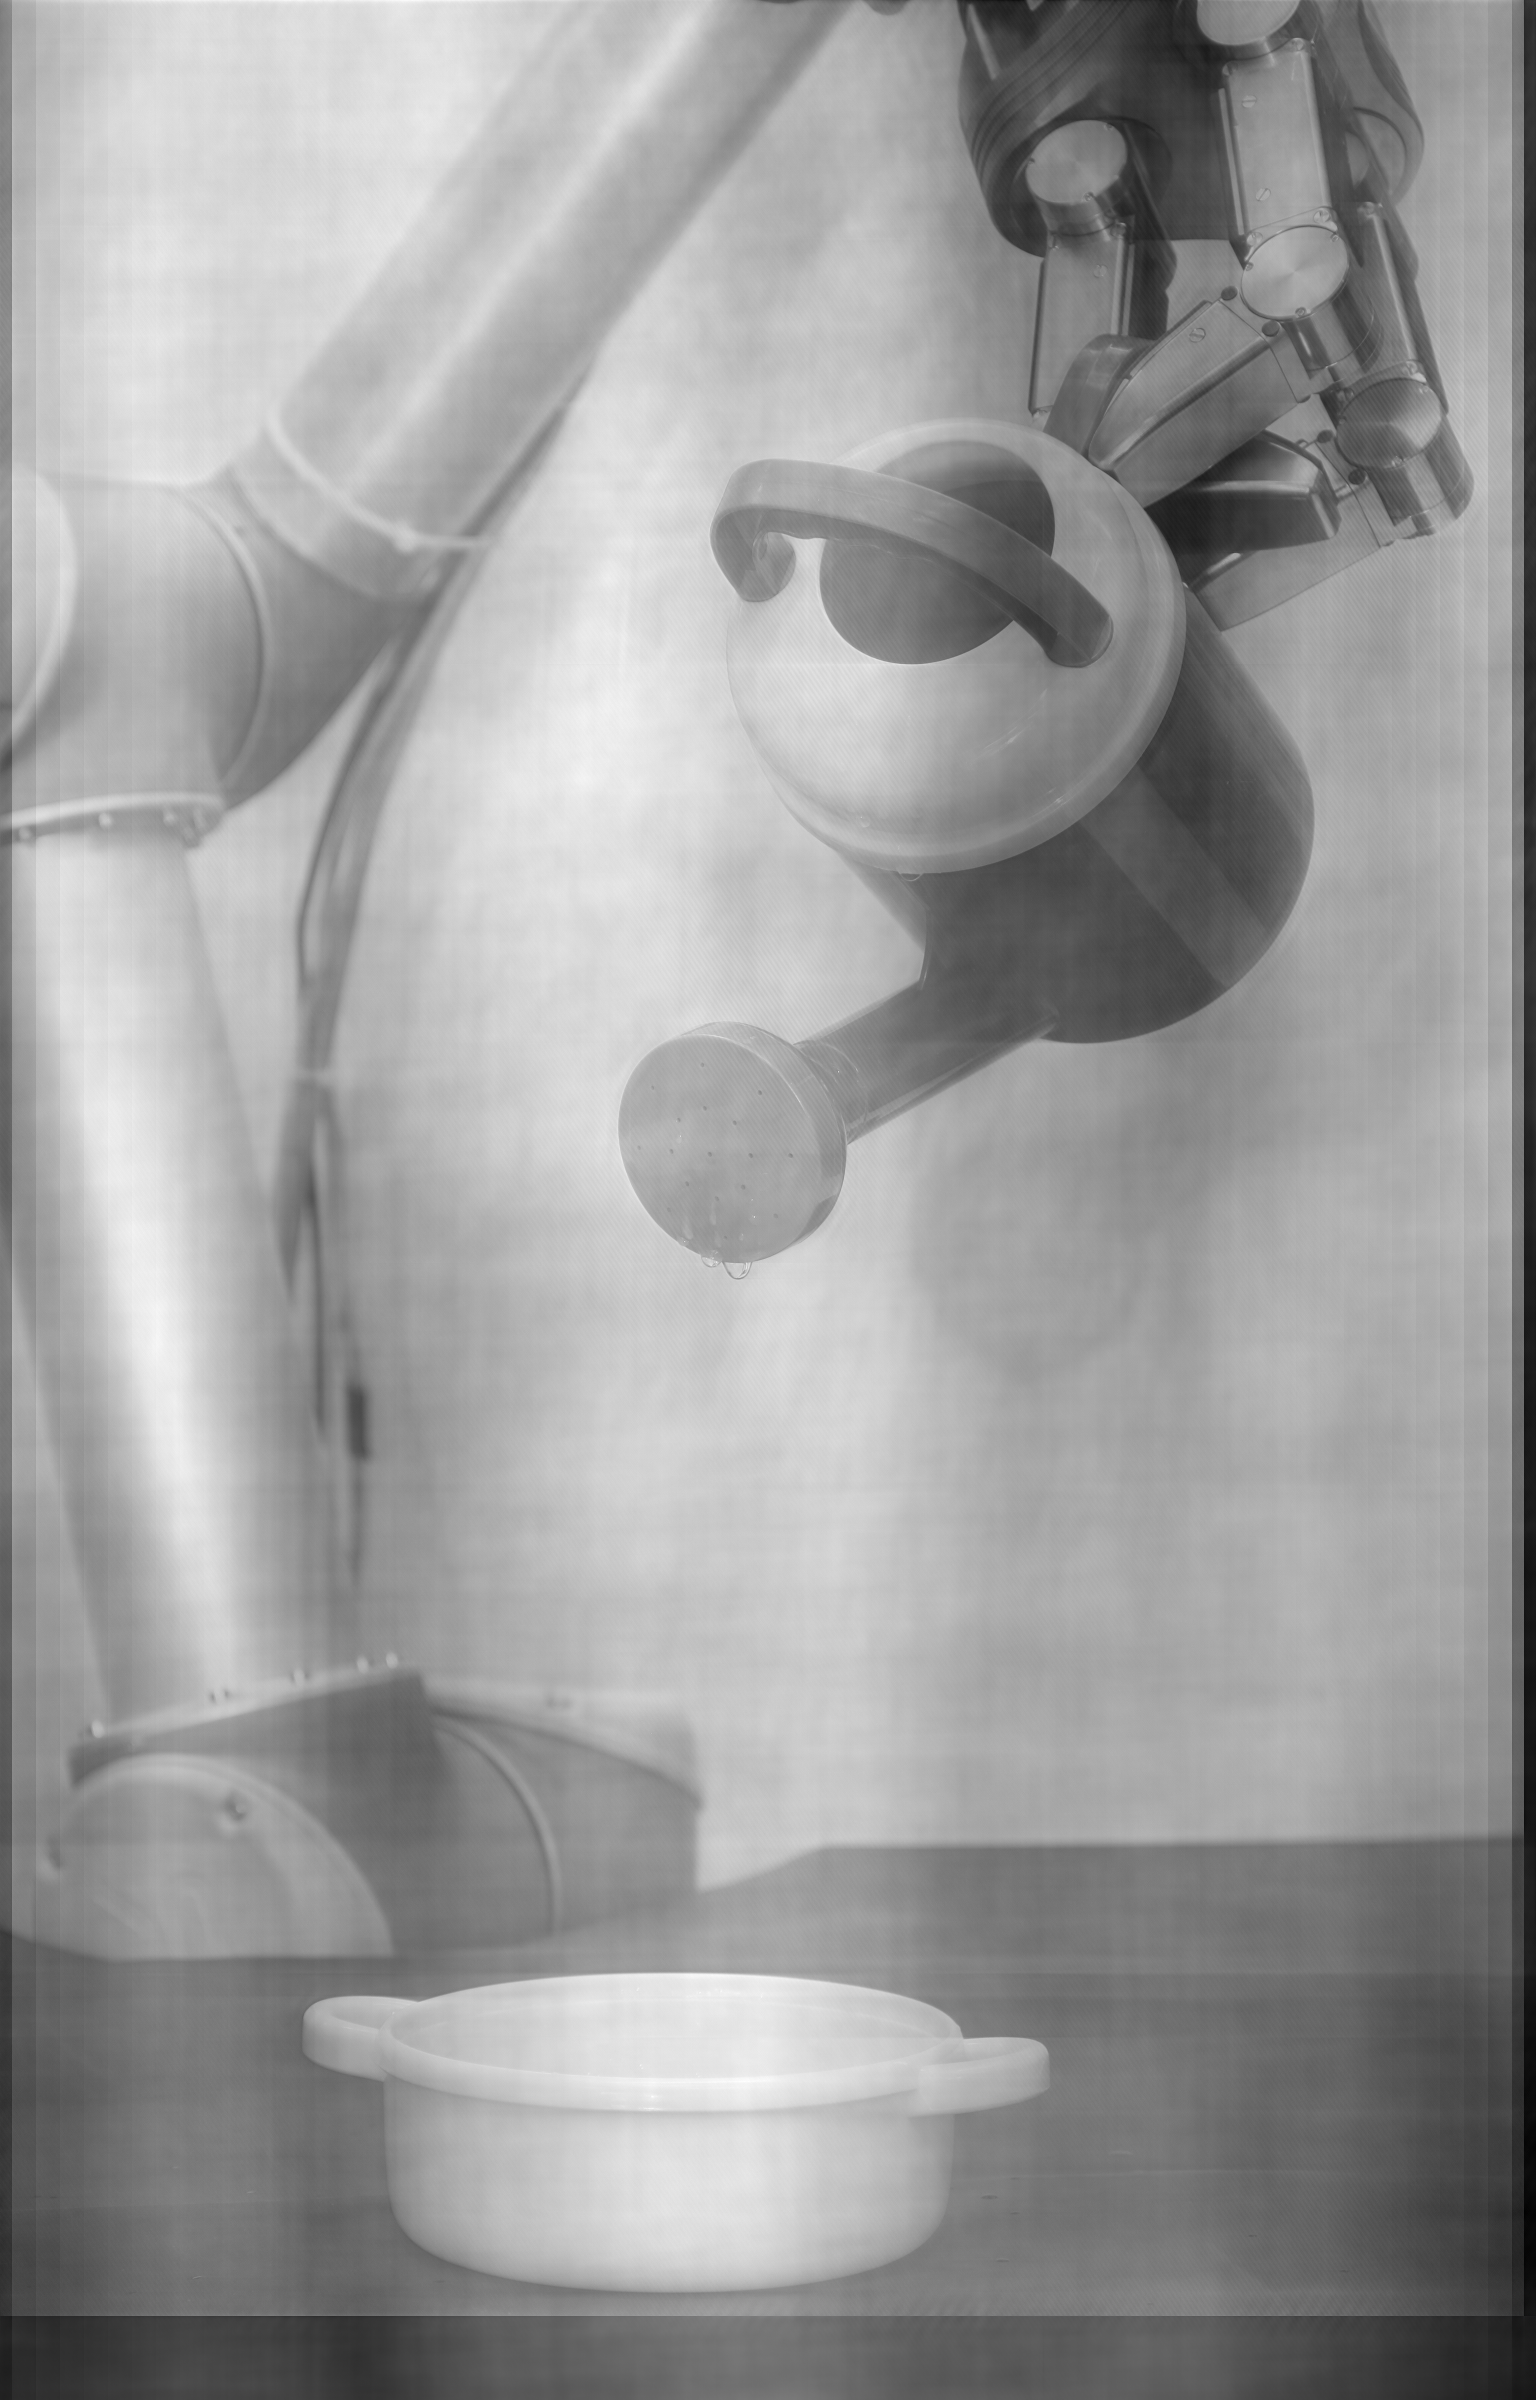
\includegraphics[width = \fullImageWidth]{../code/images/image_result_04.png}
\caption{Resulting image after filtering the disturbance from image 4.1 in the frequency domain.}
\label{fig:result_freq_04}
\end{figure}



\section{Conclusion}


\end{document}